\textbf{Pour cette première partie, aucune justification n'est demandée et une seule réponse est possible par question. Pour chaque question, reportez son numéro sur votre copie et indiquez votre réponse.}

Une réponse fausse ou l'absence de réponse n'enlève aucun point.

\subsection*{Question 1}

On considère deux réels quelconques $a$ et $b$ ainsi que le réel $E$ défini par
\[ E = -(a-b) + a - b. \]

On peut affirmer que :

\medskip
\begin{tblr}{colspec = {@{}*{4}{X}}}
	\textbf{A.}\quad $E=0$ &
	\textbf{B.}\quad $E=2a$ &
	\textbf{C.}\quad $E=2b$ &
	\textbf{D.}\quad $E=-2b$ \\
\end{tblr}

\subsection*{Question 2}

On note $S$ l'ensemble des solutions de l'équation $x^2=6$ dans $\R$.

On peut affirmer que :

\medskip
\begin{tblr}{colspec = {@{}*{2}{X}}}
	\textbf{A.}\quad $S = \left\{-\sqrt{3} ; \sqrt{3}\right\}$ &
	\textbf{B.}\quad $S = \{-3 ; 3\}$ \\
	\textbf{C.}\quad $S = \varnothing$ &
	\textbf{D.}\quad $S = \left\{-\sqrt{6} ; \sqrt{6}\right\}$ \\
\end{tblr}

\subsection*{Question 3}

Une expression développée de $(3x-5)^2$ est :

\medskip
\begin{tblr}{colspec = {@{}*{4}{X}}}
	\textbf{A.}\quad $9x^2+25$ &
	\textbf{B.}\quad $9x^2-25$ &
	\textbf{C.}\quad $3x^2-30x+25$ &
	\textbf{D.}\quad $9x^2-30x+25$ \\
\end{tblr}

\subsection*{Question 4}

\begin{minipage}[t]{0.55\linewidth}
	On a représenté ci-contre une droite dans un repère orthonormé.

	Une équation de cette droite est :

	\medskip
	\begin{tblr}{colspec = {@{}*{2}{X}}, rowsep=4pt}
		\textbf{A.}\quad $y = -\dfrac{1}{2}x+3$ &
		\textbf{B.}\quad $y = -2x+3$ \\
		\textbf{C.}\quad $y = -6x+3$ &
		\textbf{D.}\quad $y = \dfrac{3}{6}x+3$ \\
	\end{tblr}
\end{minipage}
\hfill
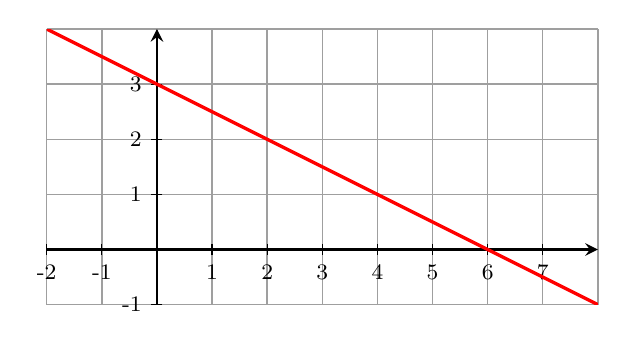
\begin{tikzpicture}[x=0.7cm,y=0.7cm,>=stealth,baseline={(current bounding box.north)}]
	\draw[step=1,gray!75,line width=0.5pt] (-2,-1) grid (8,4);
	\draw[->,line width=1pt] (-2,0) -- (8,0);
	\draw[->,line width=1pt] (0,-1) -- (0,4);
	\foreach \x in {-2,-1,1,2,3,4,5,6,7} \draw (\x,2pt) -- (\x,-2pt) node[below] {\footnotesize \np{\x}};
	\foreach \y in {-1,1,2,3} \draw (2pt,\y) -- (-2pt,\y) node[left] {\footnotesize \np{\y}};
	\clip (-2,-1) rectangle (8,4);
	\draw[line width=1.2pt,red] plot[domain=-2:8] (\x,{-0.5*\x+3});
\end{tikzpicture}

\subsection*{Question 5}

La moitié de $2^{10}$ est égale à :

\medskip
\begin{tblr}{colspec = {@{}*{4}{X}}}
	\textbf{A.}\quad $1^{10}$ &
	\textbf{B.}\quad $2^5$ &
	\textbf{C.}\quad $2^9$ &
	\textbf{D.}\quad $\left(\dfrac{1}{2}\right)^{10}$ \\
\end{tblr}



\subsection*{Question 6}

On considère la formule $a = \dfrac{1}{2}bx^2$, où $a$, $b$ et $x$ sont des réels strictement positifs.

On peut affirmer que :

\medskip
\begin{tblr}{colspec = {@{}*{4}{X}}}
	\textbf{A.}\quad $x = \sqrt{\dfrac{a}{2b}}$ &
	\textbf{B.}\quad $x = \sqrt{\dfrac{2a}{b}}$ &
	\textbf{C.}\quad $x = \dfrac{2a^2}{b}$ &
	\textbf{D.}\quad $x = \dfrac{\sqrt{a}}{2b}$ \\
\end{tblr}

\subsection*{Question 7}

On considère la fonction $f$ définie sur $\R$ par $f(x) = (2x-6)(-x+1)$.

Le tableau de signes sur $\R$ de la fonction $f$ est :

\medskip
\begin{tblr}{colspec = {@{}*{2}{X}}, rowsep=6pt}
	\textbf{A.}\quad
	\begin{tikzpicture}[baseline=(current bounding box.center)]
		\tkzTabInit[espcl=1.35]{$x$/0.8,$f(x)$/0.8}{$-\infty$,$-1$,$3$,$+\infty$}
		\tkzTabLine{,+,z,-,z,+,}
	\end{tikzpicture}
	&
	\textbf{B.}\quad
	\begin{tikzpicture}[baseline=(current bounding box.center)]
		\tkzTabInit[espcl=1.35]{$x$/0.8,$f(x)$/0.8}{$-\infty$,$1$,$3$,$+\infty$}
		\tkzTabLine{,+,z,-,z,+,}
	\end{tikzpicture}
	\\
	\textbf{C.}\quad
	\begin{tikzpicture}[baseline=(current bounding box.center)]
		\tkzTabInit[espcl=1.35]{$x$/0.8,$f(x)$/0.8}{$-\infty$,$1$,$3$,$+\infty$}
		\tkzTabLine{,-,z,+,z,-,}
	\end{tikzpicture}
	&
	\textbf{D.}\quad
	\begin{tikzpicture}[baseline=(current bounding box.center)]
		\tkzTabInit[espcl=1.35]{$x$/0.8,$f(x)$/0.8}{$-\infty$,$-3$,$1$,$+\infty$}
		\tkzTabLine{,-,z,+,z,-,}
	\end{tikzpicture}
	\\
\end{tblr}

\subsection*{Question 8}

Un prix baisse de 20\,\% puis encore de 30\,\%.

Ces deux baisses sont équivalentes à une baisse de :

\medskip
\begin{tblr}{colspec = {@{}*{4}{X}}}
	\textbf{A.}\quad 44\,\% &
	\textbf{B.}\quad 50\,\% &
	\textbf{C.}\quad 56\,\% &
	\textbf{D.}\quad 60\,\% \\
\end{tblr}
